\chapter{10 Questions with a Millionaire: Robert Miller on Cashflow, Brand, and Compounding}

This interview is organized as a set of business questions, but it has a tighter internal logic than that format first suggests. It opens with a result before we have been given the mechanism: earlier agencies shut down, yet later ventures moved faster. From there the lecture works backward and then forward again, isolating the quantities that survive failure and the quantities that do not. If we keep track of reputation, learned capability, cashflow, team alignment, learning capital, and health, the interview reads as a compact theory of entrepreneurial compounding rather than a loose set of opinions.

\begin{remark}
No validated blackboard-style frames survived for this lecture. The displayed formulas and the figure below are therefore transcript-led compressions or cautious editorial reconstructions rather than transcriptions of visible board mathematics.
\end{remark}

\section{Personal Brand as the Asset That Survives Venture Failure}

The lecture begins with a cold open, and the cold open is already a theorem in miniature. Miller says that he shut down an early agency, then another, and yet later scaled a third business to multiple seven figures within about six months. He then adds a further claim: the next business reached a seven-figure runway within about sixty days. These are speaker claims, not audited balances, but they are the right place to begin because they force the central question. How can repeated resets coexist with faster later growth?

As a bookkeeping device, we may collect the entrepreneurial state variables into
\begin{equation}
X_t=(B_t,K_t,C_t,T_t,H_t),
\end{equation}
where \(B_t\) is personal brand and market reputation, \(K_t\) is learned capability, \(C_t\) is operating cashflow, \(T_t\) is team quality and alignment, and \(H_t\) is health or usable work capacity.

\paragraph{Claim.} The venture shell may fail while the operator's accumulated market standing survives.

A cautious way to write that claim is
\begin{equation}
V_i\text{ closes } \not\Rightarrow B_{i+1}=0,
\qquad
V_i\text{ closes } \not\Rightarrow K_{i+1}=0,
\end{equation}
where \(V_i\) denotes the \(i\)-th venture form. The notation is editorial, but the idea is faithful to the opening: a particular company may end, while reputation and capability continue forward.

\paragraph{Mechanism.} The market remembers the operator even when the current offer disappears. In that sense the lecture immediately divides entrepreneurial objects into two classes:
\begin{itemize}
\item durable assets: reputation, audience trust, learned acquisition skill, judgment,
\item transient mechanisms: a specific offer, an agency shell, a partner mix, a current channel.
\end{itemize}

The rest of the chapter unfolds from this division. First we ask how Miller discovered what kind of business he needed to build. Then we ask how such a business scales. Only after that do we return to the opening puzzle and see why personal brand could carry later ventures across the gap left by earlier failures.

\section{From Capital Gains to Cashflow}

After the teaser, the interview resets into a conventional introduction. Miller places himself in three overlapping domains: digital marketing, e-commerce, and crypto. The next question then turns to college, and here the lecture makes its first sharp economic distinction.

He says that he entered college studying business administration and economics, but that the school system did not fit the career path he was actually moving toward. The decisive turn came outside the university, when he encountered digital marketing training. That matters because, by his own account, he had already made money in crypto by then. But the money had not solved the entrepreneurial problem.

The core distinction is
\begin{equation}
G \neq C,
\end{equation}
where \(G\) denotes capital gains and \(C\) denotes operating cashflow.

That is the lecture's first real mathematical move. An appreciated asset can enlarge wealth, but it does not by itself build a recurring business. Miller's point is not that gains are useless. It is that gains do not answer the question, ``How do I build cashflow?'' Once that question appears, outside education in marketing becomes legible as something more than self-help. It becomes the acquisition of a commercial mechanism.

\subsection{Question \& Answer}

\paragraph{Question.} Why can college be optional for entrepreneurship and still remain necessary for other careers?

\paragraph{Answer.} The interview's answer is structural, not merely rhetorical. Some professions trade on credentialed trust; doctors, lawyers, and similar roles need institutional pedigree. Entrepreneurship, as Miller frames it here, does not begin with pedigree but with problem-solving and the ability to create recurring revenue. College may still be useful, but it is not the essential operator in the business equation. The essential operator is the conversion of skill into cashflow.

This is why the sequence in the lecture matters. We are not simply told that college is unnecessary. We are first shown a young operator with gains on paper, then shown that those gains were insufficient, and only then shown the move toward marketing as the search for a real business.

\section{The Growth Stack: Marketing, Sales, Then Finance}

Once the cashflow problem has been posed, the lecture naturally asks what scaling actually requires. Miller's answer is ordered. It is not a bag of tactics. It is a sequence.

In transcript-backed compression,
\begin{align}
\text{Traffic} &\to \text{Leads},\\
\text{Leads} &\to \text{Sales},\\
\text{Sales} &\to \text{Revenue}.
\end{align}
He then adds the third discipline that is often delayed:
\begin{equation}
\text{Scale} \Leftarrow (M \to S \to F),
\end{equation}
where \(M\) is marketing, \(S\) is sales, and \(F\) is finance.

The lecture is careful about the first term. Marketing is not reduced to paid advertising. It includes content, traffic strategy, and the work of making people care. Sales comes next because attention is not yet revenue. Finance appears third because one cannot interpret or preserve cashflow that one has not yet learned to generate.

Because no validated diagram frame survives, the following figure is a transcript-based reconstruction of the sequence as spoken.

\begin{figure}[h]
\centering
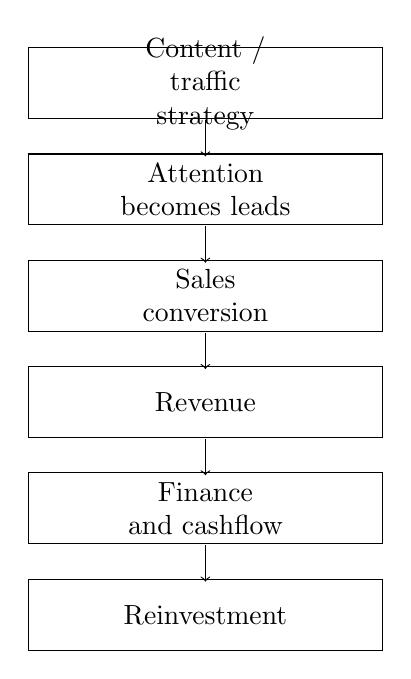
\begin{tikzpicture}[x=1cm,y=1cm]
\draw (0,0) rectangle (4.5,0.9);
\node[text width=3.7cm,align=center] at (2.25,0.45) {Content /\\ traffic\\ strategy};

\draw[->] (2.25,-0.02) -- (2.25,-0.48);

\draw (0,-1.35) rectangle (4.5,-0.45);
\node[text width=3.7cm,align=center] at (2.25,-0.90) {Attention\\ becomes leads};

\draw[->] (2.25,-1.37) -- (2.25,-1.83);

\draw (0,-2.70) rectangle (4.5,-1.80);
\node[text width=3.7cm,align=center] at (2.25,-2.25) {Sales\\ conversion};

\draw[->] (2.25,-2.72) -- (2.25,-3.18);

\draw (0,-4.05) rectangle (4.5,-3.15);
\node[text width=3.7cm,align=center] at (2.25,-3.60) {Revenue};

\draw[->] (2.25,-4.07) -- (2.25,-4.53);

\draw (0,-5.40) rectangle (4.5,-4.50);
\node[text width=3.7cm,align=center] at (2.25,-4.95) {Finance\\ and cashflow};

\draw[->] (2.25,-5.42) -- (2.25,-5.88);

\draw (0,-6.75) rectangle (4.5,-5.85);
\node[text width=3.7cm,align=center] at (2.25,-6.30) {Reinvestment};
\end{tikzpicture}
\end{figure}

The derivation is simple, but the order is everything:
\begin{enumerate}
\item Content and traffic strategy create attention.
\item Attention becomes economically useful when it yields leads.
\item Leads require sales skill before they become revenue.
\item Revenue must be interpreted through finance before it stabilizes as cashflow.
\item Only then does reinvestment become rational rather than improvised.
\end{enumerate}

This is why the lecture refuses to flatten marketing, sales, and finance into equal bullets. Finance comes last because it is downstream of demand generation and conversion. The question is not merely how to count the money. The question is how to produce the stream that can later be counted.

\section{Strategic Frameworks and the Persistence of Reputation}

At this point the host asks for book recommendations. In a weaker draft this might look like a detour, but it is not. The interview has just given us an operational stack. The book segment widens the lens from operation to judgment.

Miller's first recommendation, \emph{The Road Less Stupid}, is described in somewhat repetitive speech, but the substance is clear: it teaches one to think ahead about products, offers, and business consequences before rolling them out. \emph{Multipliers} enters next because growth is no longer only a matter of individual output; it becomes a question of how other people's efforts are amplified. \emph{Predictable Revenue} then returns the lecture to the sales problem, but now at the level of repeatable structure rather than ad hoc hustle.

From there the lecture moves directly back to the opening theme. Miller says that what one does for people will change because the market changes. Offers change. The mechanism by which sales are produced changes. Most businesses, especially in marketing and e-commerce, do not persist unchanged for generations. What persists is the operator's name in the market.

A useful update rule is
\begin{equation}
B_{t+1}=B_t+\Delta b_t,
\end{equation}
where \(\Delta b_t\) denotes the increment of reputation earned through delivery, visibility, and repeated market contact. The notation is again editorial, but it captures the lecture's actual logic. Personal brand is not treated here as decoration. It is a carry-over variable.

\subsection{Question \& Answer}

\paragraph{Question.} What actually carries forward when a company shuts down?

\paragraph{Answer.} Not the legal wrapper, not the old offer, and not necessarily the same team. What carries forward is accumulated market trust: a name, a track record, a visible history of solving a specific class of problems. The cold open becomes intelligible only when we preserve this distinction. Repeated shutdowns do not force repeated zeroes if the operator's reputation has been compounding in parallel.

That is why the lecture begins with personal brand and then later returns to it. The opening gives the result. The middle of the lecture provides the mechanism.

\section{Failure, Partnership Design, and Aligned Execution}

Once the lecture has shown what can persist individually, it turns to the question of what breaks collectively. The answer is not sentimental. Miller names coordination load, ego, and execution gaps as the central failure modes.

His explicit numerical rule is rough but memorable:
\begin{equation}
n_{\text{partners}} \lesssim 3.
\end{equation}
This is not a theorem; it is an experiential constraint. But it does real work in the chapter because it tells us that governance and coordination are not soft issues added after the fact. They are part of the venture's operating mathematics from the start.

The lecture then becomes more precise about what a partner must contribute. We may summarize the contribution profile by
\begin{equation}
P=(\text{connections},\text{people},\text{capital},\text{execution},\text{network}).
\end{equation}
This notation is a compression of his examples, not a quoted formula. Its use is simply to keep us from mistaking goodwill for functionality. A partner should bring something structurally necessary to the enterprise.

But \(P\) is not enough by itself. Miller repeatedly adds a second filter: shared values and a common destination. Under stress, one needs more than complementary tools. One needs a common answer to the questions, ``Where are we going?'' and ``What are we willing to do to get there?'' Without that alignment, the business becomes fragile precisely when it needs cohesion most.

\subsection{Question \& Answer}

\paragraph{Question.} What makes a business partner genuinely useful rather than merely pleasant to work with?

\paragraph{Answer.} In the lecture, usefulness has two tests. First, the partner must bring something the business really needs: connections, people, capital, execution, or network. Second, the partner must be aligned in values and direction. One may think of the first test as functional necessity and the second as stress survivability. Either one without the other is unstable.

This is why Miller treats execution so seriously. A name or an idea, by itself, is nearly worthless unless both sides can execute. Failure is not simply the event of losing. It is the exposure of where the structure was weak all along.

\section{Crypto as a Puzzle About Value, Then as an Origin Story}

Only after operations and partnership design have been discussed does the lecture widen into money itself. The crypto segment matters because it is not presented merely as market excitement. It is posed as a question: what do we, as a society, regard as valuable?

The conceptual tension is compactly written as
\begin{align}
V &\stackrel{?}{\propto} \text{scarcity},\\
V &\stackrel{?}{\propto} \text{scarcity}+E,
\end{align}
where \(V\) is perceived value and \(E\) is extraction or verification cost.

Miller's examples are gold and Bitcoin. Gold is not merely rare; it must be mined. Bitcoin, in his framing, is not merely scarce; it also requires real physical infrastructure and electricity to verify transactions. The point of the analogy is not to settle monetary theory once and for all. It is to sharpen the distinction between mere rarity and costly scarcity.

He also widens the frame beyond Bitcoin and Ethereum into central banks and CBDCs. The lecture there gestures toward surveillance, monetary control, and the future architecture of money. The transcript becomes rough in that region, so we should not force the argument past what is clearly stated. What remains clear is the direction of the question: where should wealth be stored, what makes a monetary object valuable, and what kind of social order follows from the answer?

\subsection{Question \& Answer}

\paragraph{Question.} Is something valuable because it is scarce, or because scarce value is backed by real cost?

\paragraph{Answer.} The lecture does not close the question; it stages it. Scarcity alone may be one basis of value. Scarcity backed by extraction or verification cost may be another. Miller treats Bitcoin and gold as parallel cases in this narrower sense. He then leaves open a further question: even if such an asset can preserve value, should it mainly be transacted with, or mainly be held?

The important thing is to keep the open character of the argument. This is Miller's framework for thinking, not a completed proof.

The lecture then narrows back to biography. Miller describes getting into crypto around 2015--2016, hearing about it through a local contact, seeing wallet sizes large enough to make the phenomenon undeniable, and entering early enough that the numbers became life-changing. He places Bitcoin roughly in the \(\$800\) to \(\$1000\) range, Ethereum around \(\$17\), and recalls a small initial stake.

\paragraph{Worked example.} In transcript-backed approximation,
\begin{align}
I_0 &\approx \$1.5\text{k}-\$2\text{k},\\
V_{4\text{ mo}} &\approx \$250\text{k}.
\end{align}
So the implied gross multiple is
\begin{equation}
m=\frac{V_{4\text{ mo}}}{I_0}\approx 125\text{--}167.
\end{equation}

The numerical jump matters, but the lecture immediately gives it a second meaning. The first financial break did not only enlarge his balance sheet. It also allowed him to explain the space to others, build books and courses, speak publicly, and discover an entrepreneurial lever hidden inside knowledge itself. Early understanding, when it is both scarce and teachable, becomes convertible into business traction.

\section{Financial Decisions, Learning Capital, Relationships, and the Evolving Why}

After the crypto origin story, the interview asks the natural paired question: what was the worst financial decision, and what was the best one? The ordering is important. First we see what a bad decision reveals under stress. Then we see what a good decision accumulates across time.

\paragraph{Anecdote.} The worst decision centers on a short-term payroll-support loan taken during a period of payment-processor strain and operational disorder. The term ``flash loan'' appears in the transcript, but here it should be treated cautiously; the context suggests an emergency payroll loan rather than a technical DeFi construction.

\subsection{Question \& Answer}

\paragraph{Question.} Why was the payroll-support loan a bad financial decision even though it was repaid quickly?

\paragraph{Answer.} Because the decisive variable was not the repayment schedule but the distribution of commitment. Miller says the loan was manageable and was paid back within about a month. What made the decision bad was that it exposed who was willing to share risk and who was not. He took liability to keep payroll moving; others in the same company did not meaningfully underwrite that move. The loan was therefore a financial act that doubled as an incentive audit.

This is one of the strongest analytical moments in the interview. A decision may be financially survivable and still be structurally wrong. The wrongness lies in what it reveals about the venture's hidden constitution.

The positive mirror image comes next. After the crypto gains, Miller says he put the remaining money into education:
\begin{equation}
I_{\text{education}} \approx \$30\text{k}-\$40\text{k}.
\end{equation}
This is not framed as consumption. It is framed as capability formation. He learned stocks, e-commerce, and marketing, not in order to become perfect in all three, but in order to become commercially versatile enough to discover the right domain and move faster inside it.

A cautious reconstruction of the compounding model is
\begin{align}
K_{t+1}&=K_t+L_t,\\
Y_{t+k}&=f\!\left(\sum_{i\le t} L_i\right),
\end{align}
where \(L_t\) is one learning input and \(Y_t\) is later revenue or business output. The point is not that the speaker literally presents such a formula. The point is that his spoken explanation has exactly this structure: many earlier learning inputs accumulate, and a later mastermind or mentorship may act as the catalyst without being the sole cause.

\subsection{Question \& Answer}

\paragraph{Question.} Why can the best investment look nonlinear, with the return appearing only after several earlier inputs have accumulated?

\paragraph{Answer.} Because the visible jump often comes at the end of a chain. Miller is explicit about this. The last mastermind may be the thing that appears to take someone from one million to seven million in revenue, but the real cause is cumulative. Earlier courses, earlier mistakes, earlier exposure, and earlier contacts all remain in the system. The final intervention matters because it arrives after the state has already been prepared.

The lecture then broadens once more. The next lesson is about relationships. Miller compresses relational seriousness into a hard test: if one had only three numbers to dial in a real emergency, which names would remain? The point is that not all social ties are equally load-bearing. As with business partners, the measure is not sentiment alone but reliability under pressure.

Health enters immediately afterward, and here the lecture again becomes quantitative. Miller describes sixteen-hour workdays, an overnighter, and then roughly twenty-four to forty-eight hours without sleep. In compact form,
\begin{equation}
t_{\text{work}} \approx 16\,\mathrm{h/day},
\qquad
t_{\text{sleep}} \approx 0
\text{ for }24\text{--}48\,\mathrm{h}.
\end{equation}
The resulting breakdown is not narrated as heroic excess. It is narrated as evidence that entrepreneurial effort has a hard biological boundary. Health is therefore not outside the model. It is one of the state variables that determines whether compounding can continue.

The final question concerns long-term motive, and the lecture closes by widening from money to identity. Miller begins with a childhood experience of lack: a mother earning roughly \(\$30\text{k}\) to \(\$40\text{k}\) a year in the Los Angeles suburbs, periods without enough food, and an early resolve never to repeat that scarcity for his own family. But he then says that the why evolves. Once food and basic provision are secured, the goal is no longer merely not to lack. The goal becomes growth in capacity, impact, and presence: to become more capable, more multifaceted, and more able to provide for family while also altering the scale of one's effect on the world.

This ending matters because it reorders the whole lecture. Revenue, brand, crypto gains, and courses are not discarded. They are subordinated. The final question is not just how to make money, but what kind of person the business is permitting one to become, and for whom the gains are being made useful.

\section{Summary}

Read in sequence, this interview gives us a coherent model of entrepreneurial compounding. The opening result becomes intelligible once we distinguish durable assets from transient mechanisms: a venture may close while reputation and capability survive. The middle of the lecture then sharpens the economic core of the argument: capital gains are not cashflow, and scaling proceeds in order from marketing to sales to finance. The later sections add the failure modes and the accelerants: too many partners, misaligned incentives, education that compounds nonlinearly, and health limits that cannot be ignored.

The lecture ends by widening the frame one last time. Business success is not treated as a self-justifying quantity. It is measured against relationships, bodily sustainability, family provision, and the evolving why that gives the whole compounding process its direction.